\documentclass{standalone}

\usepackage{graphicx}

\usepackage{tikz}

\usetikzlibrary{positioning}
\usetikzlibrary{arrows.meta}

\begin{document}

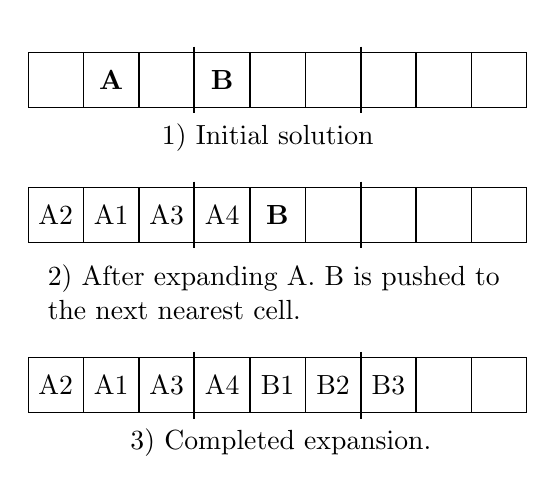
\begin{tikzpicture}[
    cell/.style={rectangle, draw, minimum width=.7cm, minimum height = .7cm},
]

% Simple expansion
\node[cell] (S11) {};
\node[cell] (S12) [right= -.01cm of S11] {\textbf{A}};
\node[cell] (S13) [right= -.01cm of S12] {};
\node[cell] (S14) [right= -.01cm of S13] {\textbf{B}};
\node[cell] (S15) [right= -.01cm of S14] {};
\node[cell] (S16) [right= -.01cm of S15] {};
\node[cell] (S17) [right= -.01cm of S16] {};
\node[cell] (S18) [right= -.01cm of S17] {};
\node[cell] (S19) [right= -.01cm of S18] {};

\node (H1) [below=0.25cm of S11] {};
\node (T1) [right=1.1cm of H1] {1) Initial solution};

\node[cell] (S21) [below=0.5cm of H1] {A2};
\node[cell] (S22) [right= -.01cm of S21] {A1};
\node[cell] (S23) [right= -.01cm of S22] {A3};
\node[cell] (S24) [right= -.01cm of S23] {A4};
\node[cell] (S25) [right= -.01cm of S24] {\textbf{B}};
\node[cell] (S26) [right= -.01cm of S25] {};
\node[cell] (S27) [right= -.01cm of S26] {};
\node[cell] (S28) [right= -.01cm of S27] {};
\node[cell] (S29) [right= -.01cm of S28] {};

\node (H2) [below=0.5cm of S21] {};
\node (T2) [right=-0.35cm of H2, text width = 6cm] {2) After expanding A. B is pushed to the next nearest cell.};

\node[cell] (S31) [below=0.7cm of H2] {A2};
\node[cell] (S32) [right= -.01cm of S31] {A1};
\node[cell] (S33) [right= -.01cm of S32] {A3};
\node[cell] (S34) [right= -.01cm of S33] {A4};
\node[cell] (S35) [right= -.01cm of S34] {B1};
\node[cell] (S36) [right= -.01cm of S35] {B2};
\node[cell] (S37) [right= -.01cm of S36] {B3};
\node[cell] (S38) [right= -.01cm of S37] {};
\node[cell] (S39) [right= -.01cm of S38] {};

\node (H3) [below=0.25cm of S31] {};
\node (T3) [right=0.7cm of H3] {3) Completed expansion.};

% Row 1
\node (SH1) [right=-.13cm of S13] {};
\node (SH2) [above=.3cm of SH1] {};
\node (SH3) [below=.3cm of SH1] {};
\draw[-, thick] (SH2) -- (SH3);

\node (SH1) [right=-.13cm of S16] {};
\node (SH2) [above=.3cm of SH1] {};
\node (SH3) [below=.3cm of SH1] {};
\draw[-, thick] (SH2) -- (SH3);

% Row 2
\node (SH1) [right=-.13cm of S23] {};
\node (SH2) [above=.3cm of SH1] {};
\node (SH3) [below=.3cm of SH1] {};
\draw[-, thick] (SH2) -- (SH3);

\node (SH1) [right=-.13cm of S26] {};
\node (SH2) [above=.3cm of SH1] {};
\node (SH3) [below=.3cm of SH1] {};
\draw[-, thick] (SH2) -- (SH3);

% Row 3
\node (SH1) [right=-.13cm of S33] {};
\node (SH2) [above=.3cm of SH1] {};
\node (SH3) [below=.3cm of SH1] {};
\draw[-, thick] (SH2) -- (SH3);

\node (SH1) [right=-.13cm of S36] {};
\node (SH2) [above=.3cm of SH1] {};
\node (SH3) [below=.3cm of SH1] {};
\draw[-, thick] (SH2) -- (SH3);

\end{tikzpicture}

\end{document}